\documentclass[tikz]{standalone}
\usepackage{tikz}
\usetikzlibrary{calc, angles, quotes}
\usetikzlibrary{intersections} % Necessário para achar pontos de cruzamento

\begin{document}

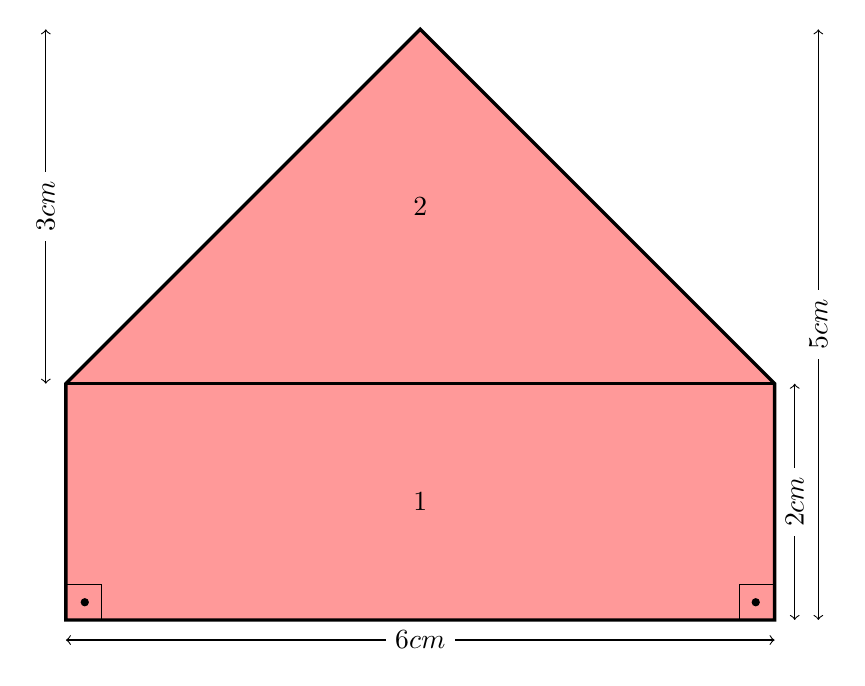
\begin{tikzpicture}[scale=1.5,rotate=90]
  \coordinate (A) at (0,0);
  \coordinate (B) at (0,6);
  \coordinate (C) at (2,6);
  \coordinate (D) at (5,3);
  \coordinate (E) at (2,0);
  \coordinate (F) at (5,0);
  \coordinate (G) at (5,6);
  
  \draw[fill=red!40,line width=1.2pt]
        (A) --
        (B) --
        (C) --
        (D) --
        (E) -- cycle;
  \draw[line width=1.2pt]
        (C) -- (E);
 
  \draw ($(A)+(3mm,0)$) -- ($(A)+(3mm,3mm)$) -- ($(A)+(0,3mm)$); 
  \draw ($(B)+(3mm,0)$) -- ($(B)+(3mm,-3mm)$) -- ($(B)+(0,-3mm)$);
  \fill ([xshift=1.5mm,yshift=1.6mm]A) circle (1pt);
  \fill ([xshift=1.5mm,yshift=-1.6mm]B) circle (1pt);
  \draw[<->] ([yshift=-3.7mm]A) -- ([yshift=-3.7mm]F) node[midway,fill=white,rotate=90] {$5cm$};
  \draw[<->] ([yshift=-1.7mm]A) -- ([yshift=-1.7mm]E) node[midway,fill=white,rotate=90] {$2cm$};
  \draw[<->] ([xshift=-1.7mm]A) -- ([xshift=-1.7mm]B) node[midway,fill=white] {$6cm$};
  \draw[<->] ([yshift= 1.7mm]C) -- ([yshift= 1.7mm]G) node[midway,fill=white,rotate=90] {$3cm$};
  \node at (1,3) {$1$};
  \node at (3.5,3) {$2$};

\end{tikzpicture}
\end{document}